
\documentclass[11pt,a4paper, twoside,openright]{article}
\usepackage{epstopdf}
\usepackage[version=3]{mhchem} % Package for chemical equation typesetting
\usepackage{siunitx} % Provides the \SI{}{} and \si{} command for typesetting SI units
\sisetup{
	load-configurations=binary,
	detect-all,
	group-digits=false,
	output-decimal-marker={,},
	per-mode=symbol,
	per-symbol=/,
	binary-units = true
}
\usepackage{graphicx} % Required for the inclusion of images
\usepackage{natbib} % Required to change bibliography style to APA
\usepackage{amsmath} % Required for some math elements 

\usepackage{multirow}
\usepackage{longtable}
\usepackage{tabto}
\usepackage{booktabs}
\usepackage[utf8]{inputenc}
%\setlength\parindent{0pt} % Removes all indentation from paragraphs

\renewcommand{\labelenumi}{\alph{enumi}.} % Make numbering in the enumerate environment by letter rather than number (e.g. section 6)

\graphicspath{{figures/}}

%\usepackage{times} % Uncomment to use the Times New Roman font

%----------------------------------------------------------------------------------------
%	DOCUMENT INFORMATION
%----------------------------------------------------------------------------------------

\title{Transmissão de uma imagem gerada na FPGA} % Title

\author{Edição 1.0}

\date{\today} % Date for the report

\begin{document}

\maketitle % Insert the title, author and date

% Please add the following required packages to your document preamble:
% \usepackage{booktabs}
\begin{table}[h!]
	\centering
	\label{my-label}
	\begin{tabular}{@{}llll@{}}
		\toprule
		\multicolumn{1}{c}{\textbf{Data}} & \multicolumn{1}{c}{\textbf{Autor}} & \multicolumn{1}{c}{\textbf{Edição}} & \multicolumn{1}{c}{\textbf{Alterações}} \\ \midrule
		10 julho 2017                     & Marisa Oliveira                    & 1.0                                 & Lançamento Inicial                       \\ \bottomrule
	\end{tabular}
\end{table}

% If you wish to include an abstract, uncomment the lines below
%\begin{abstract}
%% Abstract text
%\end{abstract}

%----------------------------------------------------------------------------------------
%	SECTION 1
%----------------------------------------------------------------------------------------

\section{Objetivo}
\section{Arquitetura}


\begin{figure}[h]
	\begin{center}
		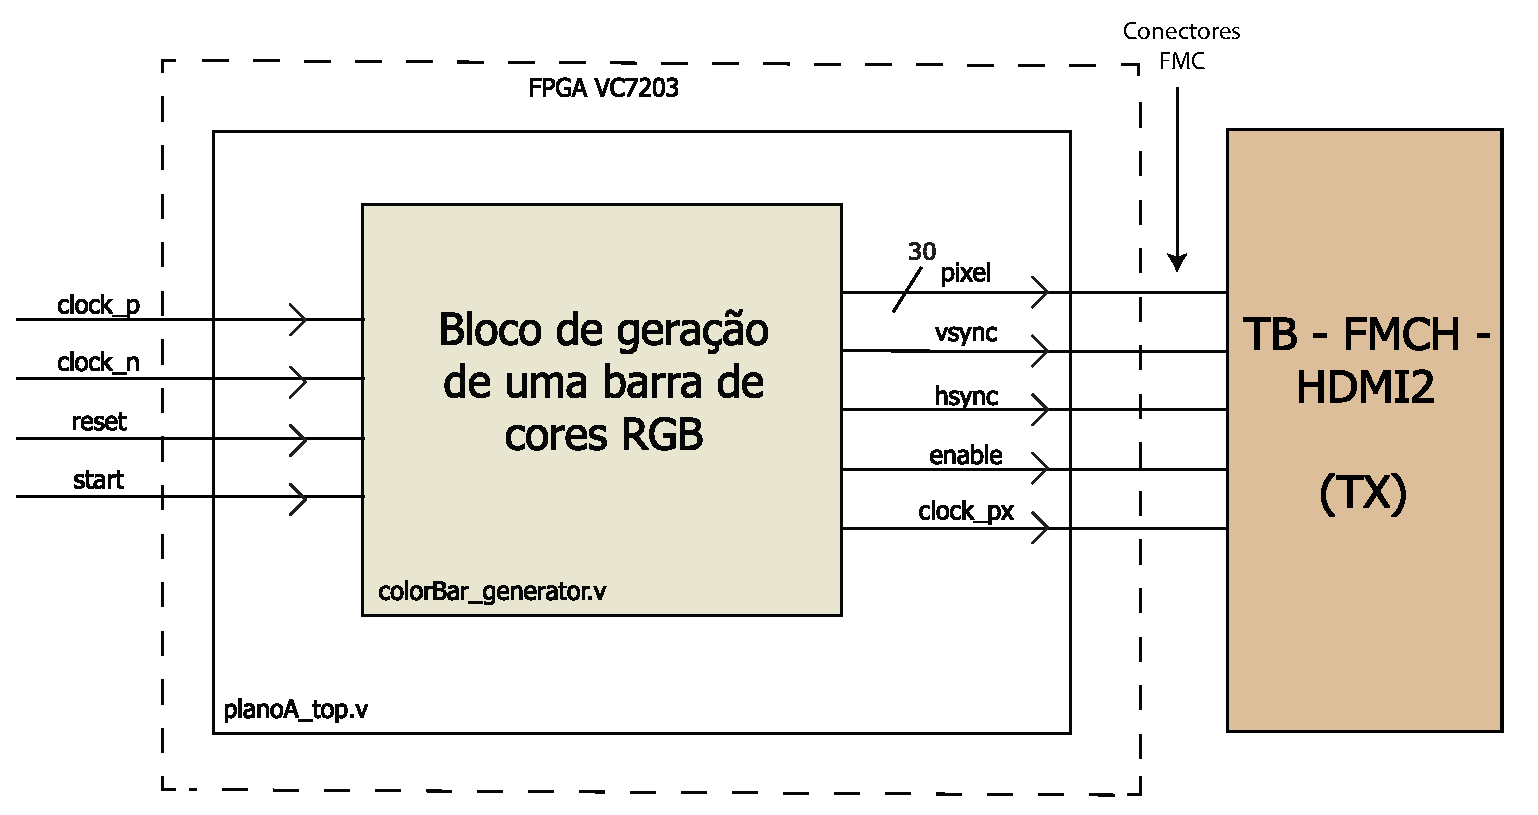
\includegraphics[width=0.65\textwidth]{planA} 
		\caption{Figure caption}
	\end{center}
\end{figure}
\section{Configuração do \textit{setup}}



%----------------------------------------------------------------------------------------
%	BIBLIOGRAPHY
%----------------------------------------------------------------------------------------

\bibliographystyle{apalike}

\bibliography{myrefs}


%----------------------------------------------------------------------------------------


\end{document}